% !TEX encoding = UTF-8
% !TEX TS-program = pdflatex
% !TEX root = ../tesi.tex
% !TEX spellcheck = it-IT

%**************************************************************
\chapter{Strumenti e tecnologie utilizzate}
\label{cap:strumenti-tecnologie}
%**************************************************************

Il contenuto di questo capitolo contiene una descrizione più dettagliata delle tecnologie e degli strumenti utilizzati per sviluppare l'applicativo oggetto dello stage.

Come anticipato nel precedente capitolo, si è scelto di utilizzare React Native come framework principale per lo sviluppo dell'applicazione, il che vincola la scelta di alcuni strumenti e tecnologie.

\section{React Native}

Trattandosi di un framework per la definizione di interfacce grafiche, React Native prevede di strutturare l'applicazione secondo \textit{compomenti}, ognuno dei quali viene definito combinando componenti standard offerti dalla libreria o altri componenti definiti dallo sviluppatore.

Visto in un ottica MVC, un componente di React Native funziona da \textit{view-controller} in quanto la definizione di un componente comprende sia la definizione dell'aspetto (\textit{view}), sia la definizione della logica di funzionamento (\textit{controller}). 

React Native offre una serie di componenti basilari che permettono di definire l'interfaccia grafica dell'applicazione e che vengono poi tradotti in componenti nativi. Questi componenti possono essere sia semplici come \texttt{View}, \texttt{Text} o \texttt{Image}, sia più complessi come \texttt{TabBarIOS} o \texttt{MapView}.

%La definizione di un componente di React Native comprende sia la definizione della logica di funzionamento, sia dell'aspetto del componente, il che riportato in un'ottica MVC, fa si che un componente sia un \textit{view-controller}, in quanto funzione sia da \textit{view} che da  \textit{controller}.

Ogni componente di un'applicazione realizzata con React Native ha sempre due proprietà:
\begin{itemize}
\item \texttt{state}: un oggetto che contiene le informazioni riguardanti lo stato del componente, la modifica di questo oggetto comporta il re-rendering dell'interfaccia grafica. Tipicamente viene utilizzato per memorizzare gli oggetti che contengono le informazioni da visualizzare sull'interfaccia grafica.
\item \texttt{props}: un oggetto che contiene le informazioni che il componente riceve dal componente che lo contiene, spesso consistono in dati da visualizzare o in funzioni di callback da invocare al verificarsi di determinati eventi. Tipicamente i campi dati di questo oggetto vengono considerati immutabili in modo da evitare \textit{side effect} indesiderati.
\end{itemize}

Questi due oggetti portano ad un pattern comune nella progettazione dei componenti detto \textit{Smart \& Dumb}, che prevede la divisione dei componenti in due categorie, quelli \textit{smart} che svolgono il ruolo di \textit{controller} dell'applicazione e quelli \textit{dumb} sono più simili a dei template.

Tipicamente un componente \textit{dumb} non ha un proprio stato e si limita a visualizzare i dati ricevuti mediante l'oggetto \texttt{props} o ad invocare delle callback al verificarsi di determinati eventi. In questo modo si ottengono dei componenti generici, indipendenti dall'applicazione che possono essere testati e riutilizzati facilmente.

Un componente \textit{smart} invece è tipicamente composto da più componenti, sia \textit{dumb} che \textit{smart}, ed è dotato di un proprio stato, contenente i dati da passare ai componenti figli.
Inoltre, un componente di questo tipo contiene la definizione delle funzioni che si occupano della gestione degli eventi.

Nel caso l'applicazione segua il design pattern Flux (§\ref{sec:flux}), i componenti \textit{smart} sono quelli che si occupano di recuperare lo stato dagli \textit{stores} e di creare le varie \textit{actions}.

Un altro pattern comune nelle applicazioni sviluppate con React Native è quello di definire un singolo componente per ogni file di codice che deve contenere tutto il codice del componente, sia quello riguardante la logica di funzionamento, sia quello riguardante la logica di layout.
Questo è reso possibile dal fatto che le informazioni riguardati lo stile sono definite come oggetti JavaScript e il layout viene definito utilizzando la sintassi JSX.

\subsection{La sintassi JSX}

La sintassi JSX permette di inserire all'interno del codice JavaScript alcuni pezzi di codice XML, che devono essere poi trasformati in JavaScript normale per poter essere eseguiti.

Il vantaggio offerto da questa sintassi è quello di poter definire in modo dichiarativo come i vari componenti dell'applicazione si compongono tra loro, semplificando così la definizione dell'interfaccia grafica.

\begin{lstlisting}[language=JavaScript, caption=Esempio della sintassi JSX di React Native]
render(){
return (
<View style={styles.container}>
  <Text style={styles.welcome}>
    Welcome to React Native!
  </Text>
  <Text style={styles.instructions}>
    To get started, edit index.ios.js
  </Text>
  <Text style={styles.instructions}>
    Press Cmd+R to reload,{'\n'}
    Cmd+D or shake for dev menu
  </Text>
</View>);
}
\end{lstlisting}

Nell'esempio sopra riportato viene definito il layout di un componente e, grazie alla sintassi derivata dall'XML, è facile intuire da quali elementi è composto e come questi elementi sono combinati tra loro.     

Nel caso di React Native la traduzione da JSX a JavaScript viene fatta dal \textit{packager} prima della compilazione dell'applicazione (§\ref{sec:packager}).

\subsection{Oggetti JavaScript per la definizione dello stile}

Con React Native la definizione dello stile dei componenti di un'applicazione viene effettuata utilizzando degli oggetti JavaScript che hanno dei campi dati simili alle proprietà dei CSS.

Questa scelta è stata effettuata perché il team di sviluppo di React Native ha dovuto implementare un sistema che trasformi le proprietà CSS in attributi dei componenti nativi ed ha ritenuto più comodo utilizzare degli oggetti JavaScript.

In questo modo vengono risolti alcuni problemi dei CSS, come la località dei nomi delle classi e la gestione delle variabili.
Inoltre, non è più necessario riferirsi ad una determinata classe CSS utilizzando una stringa, in quanto basta usare il campo dati di un oggetto JavaScript, evidenziando così eventuali errori, come l'utilizzo di un nome della classe errato.

Per creare uno di questi oggetti è necessario utilizzare le StyleSheet API messe a disposizione da React Native.

Queste API sono racchiuse all'interno del modulo \texttt{StyleSheet} e, mediante il metodo \texttt{create}, permettono di creare un oggetto che definisce lo stile di un componente a partire da un normale oggetto JavaScript.

\begin{lstlisting}[language=JavaScript, caption=Esempio della definizione dello stile di un componente di React Native]
var styles = StyleSheet.create({
  container: {
    flex: 1,
    justifyContent: 'center',
    alignItems: 'center',
    backgroundColor: '#F5FCFF',
  },
  welcome: {
    fontSize: 20,
    textAlign: 'center',
    margin: 10,
  },
  instructions: {
    textAlign: 'center',
    color: '#333333',
    marginBottom: 5,
  },
});
\end{lstlisting}

Le impostazioni delle stile sono analoghe a quelle offerte dai CSS ed includono alcune funzionalità che non sono ancora pienamente supportate nell'ambio web come il sistema di layout flexbox.
Questo sistema prevede che un componente dell'applicazione possa andare a modificare le dimensione dei componenti che contiene, in modo da occupare al meglio lo spazio disponibile e di allineare in vari modi i componenti contenuti.

\subsection{JavaScript ES6 e ES7}

Il codice JavaScript prodotto utilizzando React Native segue lo standard ES5 dal momento che è lo standard supportato dalla versione attuale di JavaScriptCore.

Tuttavia è possibile utilizzare alcune funzionalità specifiche degli standard ES6 e ES7, come la destrutturazione degli oggetti e l'utilizzo delle classi, dal momento che il \textit{packager} di React Native (§\ref{sec:packager}), prima di compilare l'applicazione nativa, compila il codice JavaScript utilizzando Babel\footnote{\url{https://babeljs.io/}}, un compilatore per JavaScript che trasforma la sintassi ES6 e ES7 in modo che sia conforme allo standard ES5.

\subsection{Animazioni}
Le animazioni sono una delle caratteristiche principali dell'esperienza d'uso delle applicazioni mobile e la fluidità delle animazioni è uno dei fattori che differenzia le applicazioni native da quelle ibride.

Per la creazione delle animazioni React Native offre due moduli: \texttt{LayoutAnimation}, per le animazioni riguardanti le modifiche al layout dei componenti, e \texttt{Animated}, per definire animazioni personalizzate e specifiche per alcuni componenti.

Entrambi questi moduli sono realizzati completamente in JavaScript e quindi non usufruiscono delle funzionalità offerte dalla piattaforma nativa. 
Nonostante ciò la fluidità delle animazioni può essere paragonabile a quella di un'applicazione nativa.

Come già anticipato, il modulo \texttt{LayoutAnimation} permette di effettuare in modo animato le modifiche subite dal layout a causa dell'esecuzione delle funzione di rendering dei componenti.
Questo, in combinazione con il sistema di layout flexbox, permette di ottenere animazioni come la comparsa o scomparsa di una barra laterale o il ridimensionamento animato dei componenti con una sola riga di codice, senza dover andare a modificare le dimensioni dei vari componenti.

\begin{lstlisting}[language=JavaScript, caption=Utilizzo di LayoutAnimation]
_onPress() {
  LayoutAnimation.spring(); //Imposta l'esecuzione della prossima funzione di rendering in modo animato
  this.setState({...}): //Modifica lo stato del componente in modo da causarne il re-rendering
}
\end{lstlisting}

Il modulo \texttt{Animated} permette invece di andare a definire animazioni più complesse, sfruttando dei componenti ad hoc il cui layout può essere definito utilizzando particolari valori che quando vengono modificati, producono un'animazione.
Un tipico utilizzo di questa tipologia di animazioni è quello di spostare alcuni elementi grafici in base ad un \gls{pan} effettuato dall'utente.

Le animazioni definite con questo modulo possono poi essere collegate tra loro, in modo da ottenere animazioni complesse come quelle legate al \gls{pinch-to-zoom} su un'immagine.

\subsection{Componenti esterni}

React Native supporta la gestione dei moduli secondo lo standard CommonJS\footnote{\url{http://requirejs.org/docs/commonjs.html}}, questo permette di utilizzare npm per la gestione delle dipendenze con i componenti esterni.

Sfruttando le possibilità offerte da npm, la community di sviluppatori ha già iniziato a pubblicare alcuni componenti per le applicazioni di React Native, che possono essere facilmente integrati nella propria applicazione.
Una raccolta di questi componenti può essere trovata sul sito React Parts\footnote{\url{https://react.parts/native-ios}}, il qualche contiene componenti sia per React che per React Native.

\subsection{Creazione di un progetto}

Per creare un'applicazione con React Native è necessario installare l'interfaccia a riga di comando che è disponibile come pacchetto npm con il nome di \texttt{react-native-cli}.

Una volta installata questa interfaccia è possibile creare un progetto con il comando \texttt{react-native init <NomeProgetto>}, il quale si occupa di creare una cartella contenente tutto il necessario per il funzionamento dell'applicazione.

Tra i vari file creati è possibile trovare il progetto di Xcode, il quale contiene tutto il codice Obj-C necessario all'esecuzione dell'applicazione.

Per avviare l'applicazione è sufficiente aprire il progetto, selezionare il simulatore o un dispositivo e premere il pulsante \textit{Play}, dopo un po' verrà avviata l'applicazione.

\subsection{Packager}\label{sec:packager}

Il \textit{Packager} è un programma presente all'interno di React Native che permette di creare dei bundle JavaScript contenenti il codice dell'applicazione.

Quando richiesto, il \textit{Packager} esegue la conversione da JSX in JavaScript, trasformando anche il JavaScript ES6 in JavaScript ES5 e successivamente crea un bundle, unendo tutti i file JavaScript necessari al funzionamento dell'applicazione.

Il bundle deve poi essere aggiunto al progetto Xcode in modo che sia disponibile sul dispositivo.

Durante lo sviluppo è inoltre possibile configurare l'applicazione in modo che il bundle con il codice JavaScript venga recuperato da un server presente nel computer con il quale si sta sviluppando.

Così facendo è possibile eseguire ogni volta il codice aggiornato senza dover reinstallare l'applicazione sul dispositivo o sul simulatore.
Il progetto Xcode che viene creato dall'interfaccia a riga di comando è configuarato in modo che avvi in modo automatico questo server.

\subsection{Developer Menu}

Durante lo sviluppo di un'applicazione con React Native è possibile accedere ad alcune funzionalità messe a disposizione dal framework per facilitare lo sviluppo delle applicazioni.

Queste funzionalità sono accessibili durante l'esecuzione dell'applicazione, indipendentemente dal fatto questa sia in esecuzione sul simulatore o su un dispositivo reale.

Per far comparire il menù quando l'applicazione viene eseguita sul simulatore è necessario premere i tasti \texttt{Cmd}+\texttt{D}, mentre se l'applicazione viene eseguita su un dispositivo reale è necessario scuotere il dispositivo.

\begin{figure}[htp]
\centering
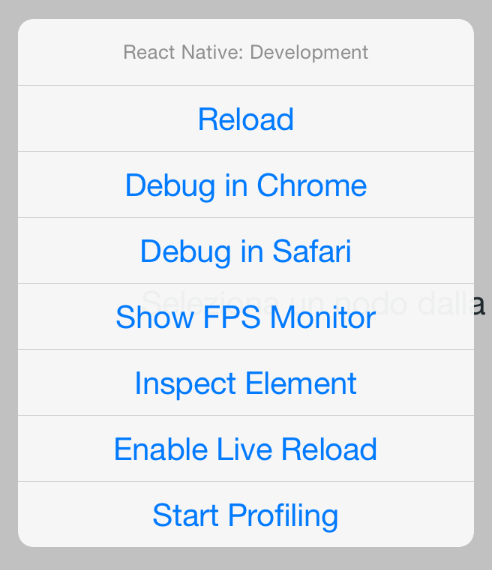
\includegraphics[width=\textwidth*1/3]{../immagini/rn-devmenu}
\caption{Developer menu di React Native}  
\end{figure}

Il menù è composto dalle voci:
\begin{itemize}
\item \textbf{Reload}: permette di ricaricare il bundle dell'applicazione.
\item \textbf{Debug in ...}: permette di eseguire il debug dell'applicazione utilizzando Chrome o Safari, maggiori informazioni sono disponibili nella sezione §\ref{sec:chrome}.
\item \textbf{Show FPS Monitor}: permette di visualizzare il numero di FPS dell'interfaccia grafica dell'applicazione.
\item \textbf{Inspect Element}: permette di analizzare i vari componenti dell'interfaccia grafica, visualizzando, per ogni componente selezionato, i componenti che lo contengono, lo stile del componente e le dimensioni effettive del componente.
\item \textbf{Enable Live Reload}: quando abilitato l'applicazione viene ricaricata in modo automatico ad ogni modifica subita dai file sorgenti.
\item \textbf{Start Profiling}: permette di visualizzare gli stack delle chiamate durante l'esecuzione dell'applicazione, relativi sia alla parte Obj-C, sia alla parte JavaScript. 
\end{itemize}

Questo menù viene rimosso automaticamente quando l'applicazione viene compilata per essere pubblicata nello store.

\section{Flux}\label{sec:flux}
Flux è un pattern architetturale per le applicazioni sviluppate con React e React Native proposto da Facebook.

L'obiettivo di questo pattern è quello di organizzare la gestione dei dati dell'applicazione in modo che ci sia un flusso di dati unidirezionale sfruttando il sistema di composizione dei componenti di React.

Il flusso parte da degli oggetti \textit{stores}, che contengono i dati dell'applicazione, questi dati vengono poi prelevati da alcuni  componenti \textit{smart} dell'applicazione, che a loro volta li forniscono ai componenti che li compongono.

Per modificare i dati presenti in uno \textit{store} è necessario creare un oggetto \textit{action} che, mediante il \textit{dispatcher} dell'applicazione, viene ricevuto dai vari \textit{stores}, i quali lo utilizzano per aggiornare i dati che contengono.

%Quando un componente vuole modificare i dati presenti in uno \textit{store}, deve creare un oggetto \textit{action} che, mediante il \textit{dispatcher} dell'applicazione, viene ricevuto dai vari \textit{stores}, i quali lo utilizzano per aggiornare i dati che contengono.

\begin{figure}[htp]
\centering
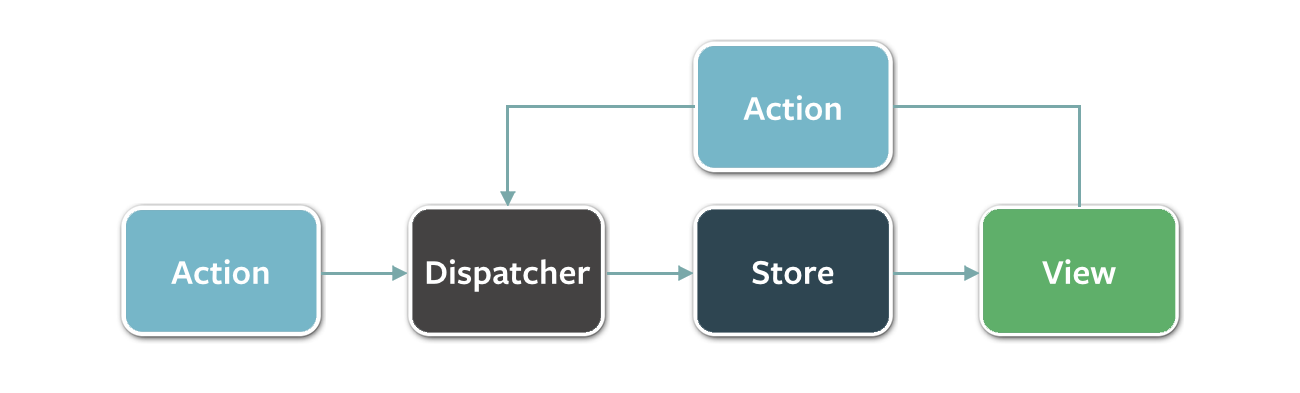
\includegraphics[width=\textwidth*3/4]{../immagini/flux-simple}
\caption{Diagramma del pattern Flux}  
\end{figure}
\FloatBarrier

Come anticipato, Flux prevede tre tipologie principali di componenti:
\begin{itemize}
\item \textbf{Stores:} sono dei \gls{singleton} che contengono i dati dell'applicazione e che forniscono solamente dei metodi \textit{getter} per recuperarli. Una volta creati, gli \textit{stores} restano in attesa dell'esecuzione di un \textit{action}, la quale può essere utilizzata per aggiornare i dati contenuti nello \textit{store}.
\item \textbf{Actions:} sono degli oggetti che contengono delle informazioni riguardante alle varie operazioni che possono eseguite dagli \textit{stores} dell'applicazione. Tipicamente vengono create dai \textit{view-controller} di React e contengono già i dati necessari agli \textit{stores} per aggiornarsi. Nel caso di operazioni asincrone i \textit{view-controller} creano l'azione che verrà comunicata al \textit{dispatcher} solamente quando le istruzioni asincrone sono state completate.
\item \textbf{Dispatcher:} oggetto che riceve un \textit{action} e ne esegue il broadcast verso tutti gli \textit{stores} dell'applicazione. Fornisce delle funzionalità che permettono ai vari \textit{stores} di registrarsi e di specificare eventuali dipendenze verso altri \textit{stores}, in modo che un determinato \textit{store} venga aggiornato una volta completato l'aggiornamento degli \textit{stores} da cui dipende, evitando così di ottenere uno stato inconsistente.


%che l'aggiornamento di un determinato \textit{store} venga effettuato solamente quando gli \textit{stores} da cui dipende abbiano finito di aggiornarsi, evitando così di ottenere uno stato inconsistente.
\end{itemize}


\subsection{Sequenza delle azioni}

\begin{figure}[htp]
\centering
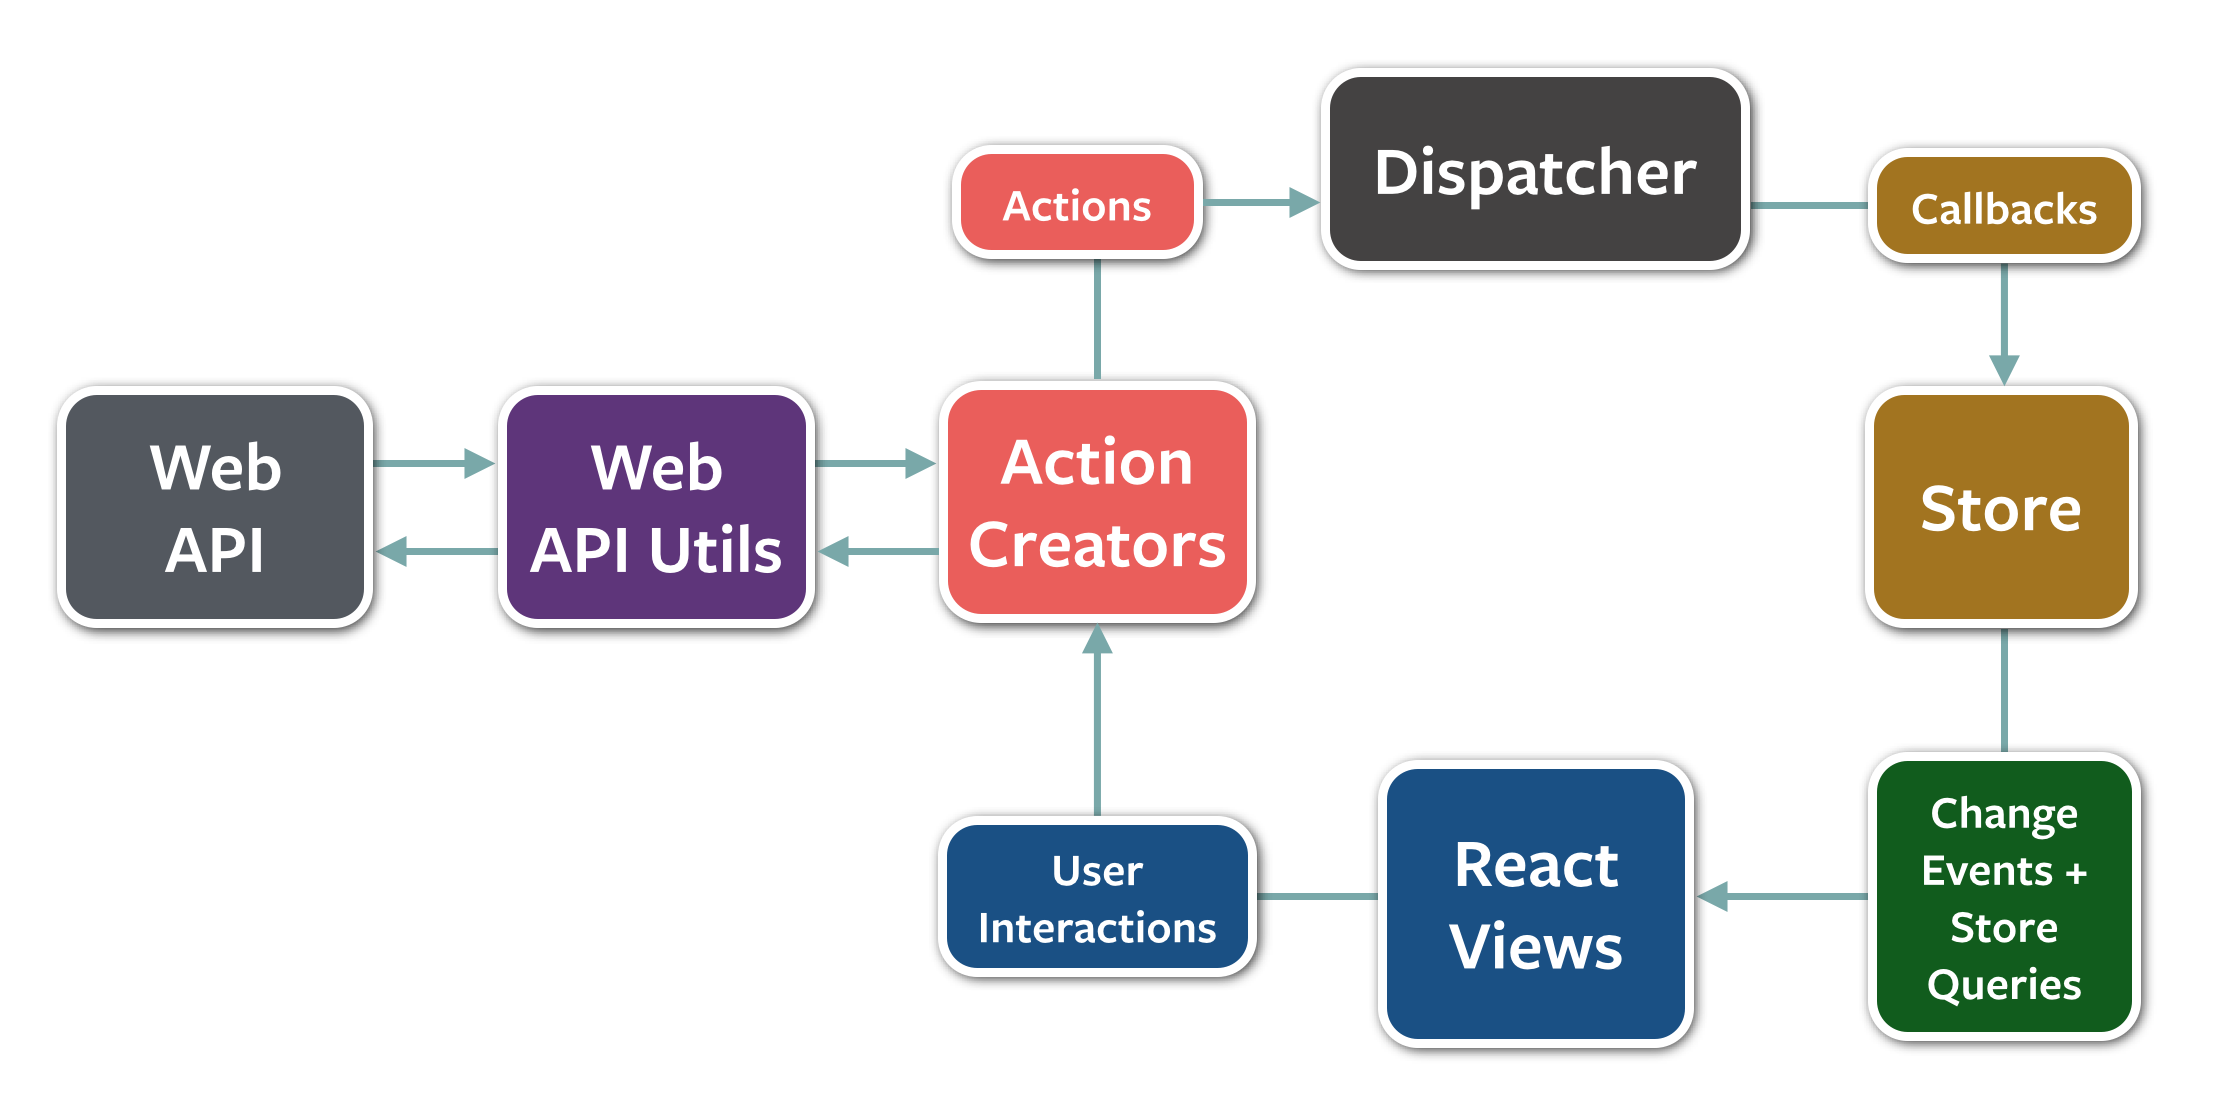
\includegraphics[width=\textwidth*3/4]{../immagini/flux-diagram}
\caption{Funzionamento del pattern Flux}  
\end{figure}
\FloatBarrier

\begin{enumerate}
\item L'utente esegue un'azione sulla view.
\item Il gestore dell'evento crea un \textit{action} e la comunica al \textit{dispatcher}.
\item Il \textit{dispatcher} manda a tutti gli \textit{stores} registrati l'oggetto \textit{action} ricevuto.
\item Ogni \textit{store} esamina l'oggetto  \textit{action} e se necessario si aggiorna. 
\item Gli \textit{stores} che hanno subito modifiche emettono un evento per comunicare ai componenti React in ascolto che si devono aggiornare.
\item I componenti React richiedono agli \textit{stores} i dati per aggiornarsi.
\end{enumerate}

\subsection{Differenze con MVC}

Nonostante Flux ed MVC possano sembrare due pattern totalmente diversi, in realtà Flux è una variante del MVC classico con delle modifiche che lo adattano al funzionamento di React e React Native.

Infatti, con MVC, i \textit{controllers} interagiscono con il \textit{model} e le \textit{view} dell'applicazione visualizzano i dati presenti nel \textit{model}.
Quando il \textit{model} viene modificato, le \textit{view} vengono notificate e recuperano i dati aggiornati dal model.

Mentre con Flux, i \textit{view-controller} aggiornano il model, definito dagli \textit{stores}, in un modo più strutturato utilizzando le \textit{actions} e, una volta che l'aggiornamento degli \textit{store} è completato, i \textit{view-controller} vengono notificati in modo che possano recuperare i nuovi dati.

Considerando che per React e React Native una \textit{view} e il relativo \textit{controller} sono rappresentati da un unico componente, diventa chiaro che la logica di base è la stessa, l'unica differenza è come viene effettuato l'aggiornamento dei dati, che con Flux deve passare attraverso delle \textit{actions}.

Questo vincolo imposto dall'utilizzo delle \textit{actions} permette di circoscrivere la logica di aggiornamento del \textit{model} all'interno del \textit{model} stesso, limitando la complessità dell'applicazione, che nel caso di grandi applicazioni può diventare ingestibile.

Un altro vantaggio che viene dall'adozione di Flux con React riguarda l'aggiornamento dell'interfaccia grafica a seguito di una modifica dei dati, in quanto sia React che Flux ragionano a stati: con React l'interfaccia grafica visualizza uno stato dell'applicazione e un cambiamento dello stato comporta il re-rendering dell'interfaccia, mentre con Flux l'insieme degli \textit{stores} rappresenta lo stato dell'applicazione e l'esecuzione di un'azione comporta il cambiamento dello stato.

Di conseguenza è possibile collegare direttamente lo stato definito dagli \textit{stores}, con lo stato dei componenti grafici, limitando il numero di operazioni intermedie.

\subsection{flux}\label{sec:flux-npm}

\texttt{flux} è un modulo pubblicato su npm da Facebook che fornisce delle classi che aiutano nell'implementazione del pattern Flux.
Tra queste classi è presente l'implementazione completa di un \textit{dispatcher} e una classe base per la creazione degli \textit{stores} che si occupa di implementare tutta la parte relativa alla registrazione e pubblicazioni degli eventi legati all'aggiornamento dei dati.


\section{Atom e Nuclide}

Trattandosi di codice JavaScript è possibile utilizzare un qualsiasi editor di testo per sviluppare l'applicazione.
Tuttavia viene consigliato l'utilizzo di Atom, un editor open source sviluppato di GitHub, che può essere personalizzato mediante dei pacchetti.

Tra i pacchetti disponibile per Atom c'è Nuclide\footnote{\url{http://nuclide.io/}} una serie di pacchetti che aggiungo alcune funzionalità di supporto allo sviluppo con React Native, come l'auto-completamento delle keyword e l'evidenziazione della sintassi JSX.

\section{Xcode}

Nonostante il codice JavaScript possa essere scritto con qualsiasi editor di testo, è necessario utilizzare Xcode\footnote{Xcode è disponibile solamente per Mac OS X, tuttavia è possibile sviluppare applicazioni con React Native su qualsiasi sistema operativo grazie ad Exponent \url{http://exponentjs.com/}. Il funzionamento di questo servizio non è stato approfondito in quanto è stato possibile utilizzare Xcode.} per compilare l'applicazione finale in modo da poterla installare sul simulatore di iOS o su un dispositivo Apple.

Xcode rende disponibili un serie di tools per lo sviluppo delle applicazioni native che possono essere riutilizzati durante lo sviluppo di un'applicazione con React Native. Ad esempio durante l'esecuzione dell'applicazione sul simulatore di iOS è possibile controllare il consumo della memoria, il traffico dati e l'utilizzo della CPU.

\begin{figure}[htp]
\centering
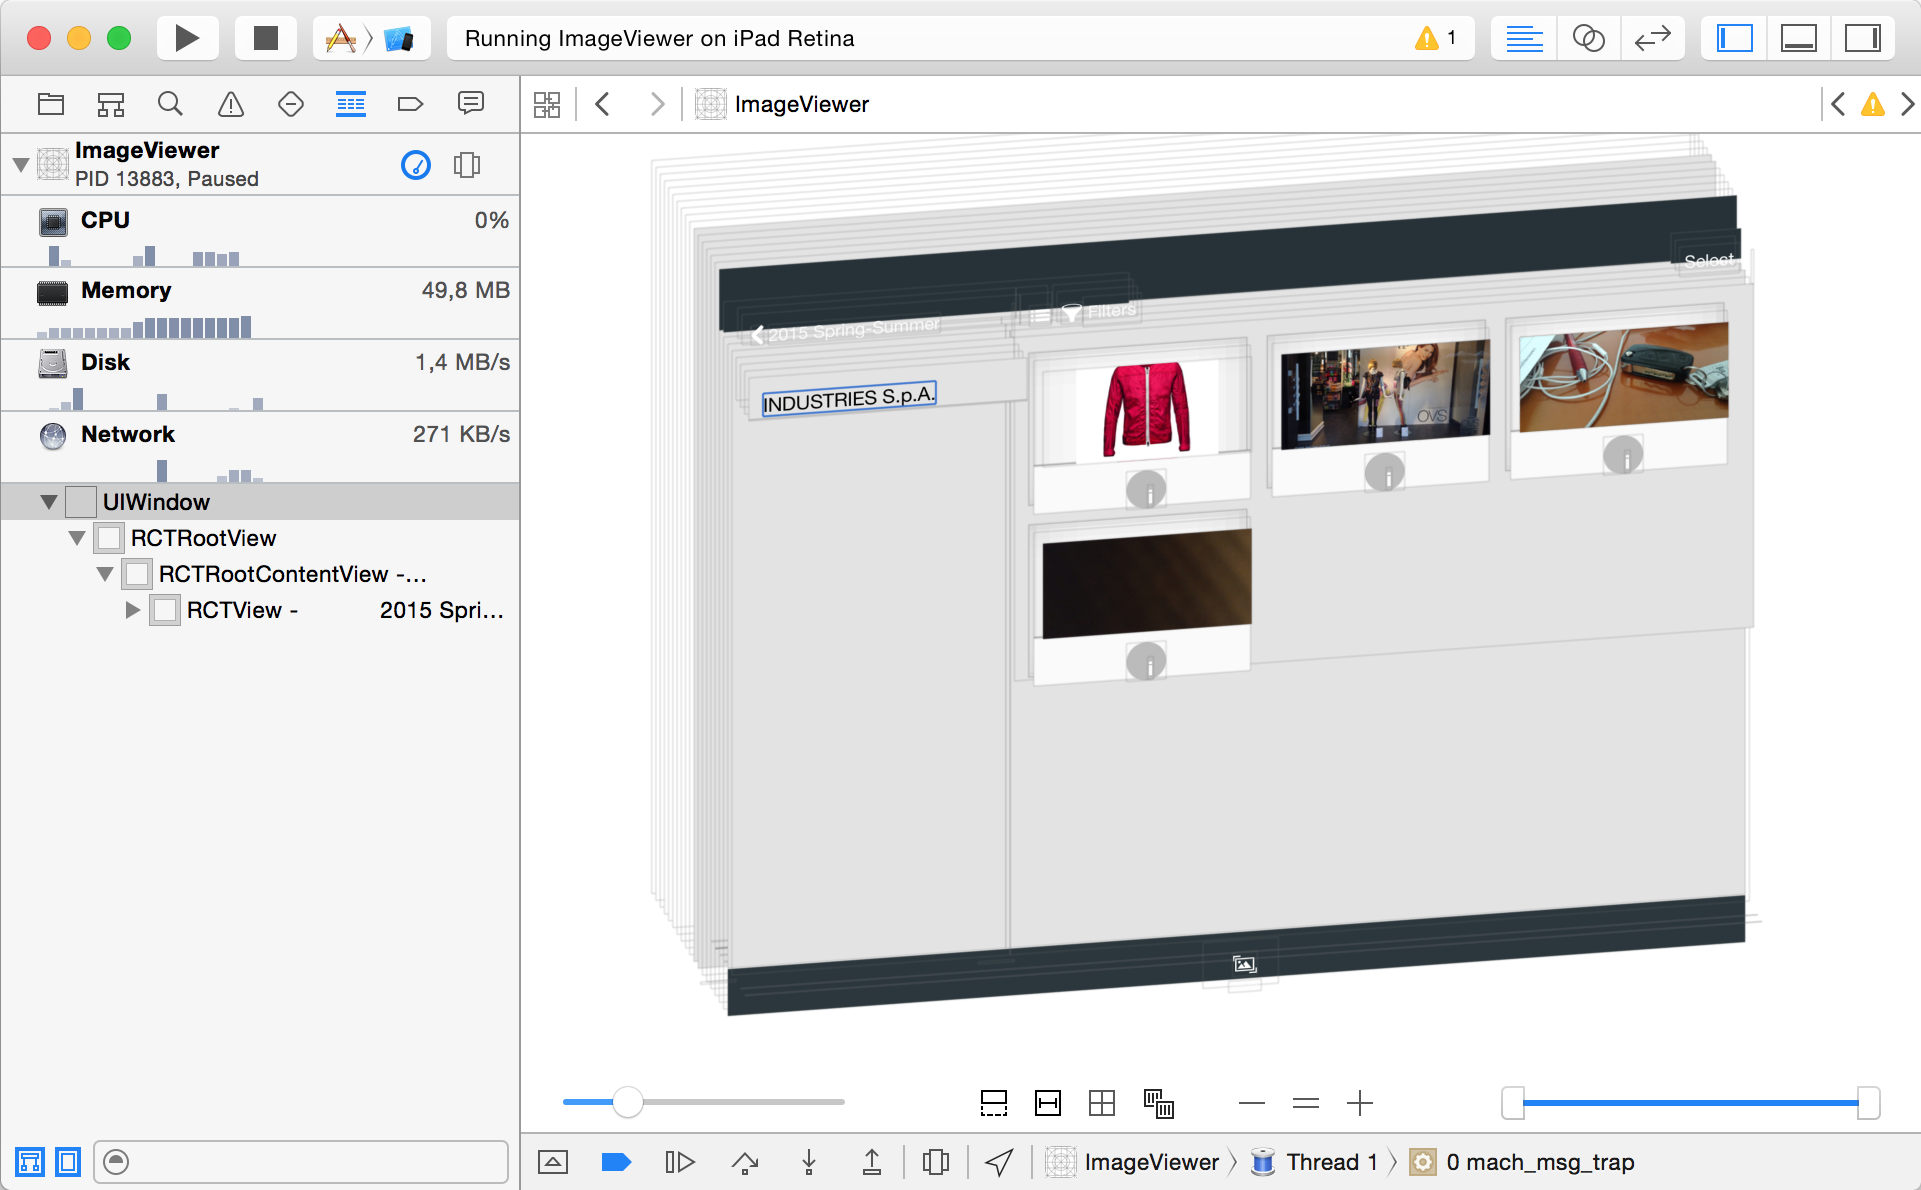
\includegraphics[width=\textwidth]{../immagini/xcode-tools}
\caption{Tools di debug di Xcode}  
\end{figure}
\FloatBarrier

\section{Google Chrome Dev Tools}\label{sec:chrome}

Durante lo sviluppo di un'applicazione con React Native è possibile utilizzare gli strumenti di sviluppo offerti da Google Chrome per effettuare il debug del codice JavaScript.

In particolare è possibile utilizzare il debugger di Chrome per inserire dei break point nel codice dell'applicazione ed effettuare l'esecuzione passo passo del codice, oppure è possibile stampare sulla console di Chrome mediante l'istruzione \texttt{console.log}.

Al momento non è possibile utilizzare tutti i tools in quanto la modalità debug di React Native utilizza una virtual machine diversa per eseguire il JavaScript.

Infatti, durante l'esecuzione normale il JavaScript viene interpretato da JavaScriptCore, mentre, durante il debug, viene utilizzata la virtual machine V8 presente all'interno di Chrome, il quale comunica con l'applicazione nativa mediante WebSocket.

In questo modo Chrome riesce a controllare l'esecuzione del JavaScript, ma non riesce ad accedere alle funzionalità che vengono eseguite dai componenti nativi, come l'utilizzo delle risorse di rete o la gestione della memoria.

\begin{figure}[htp]
\centering
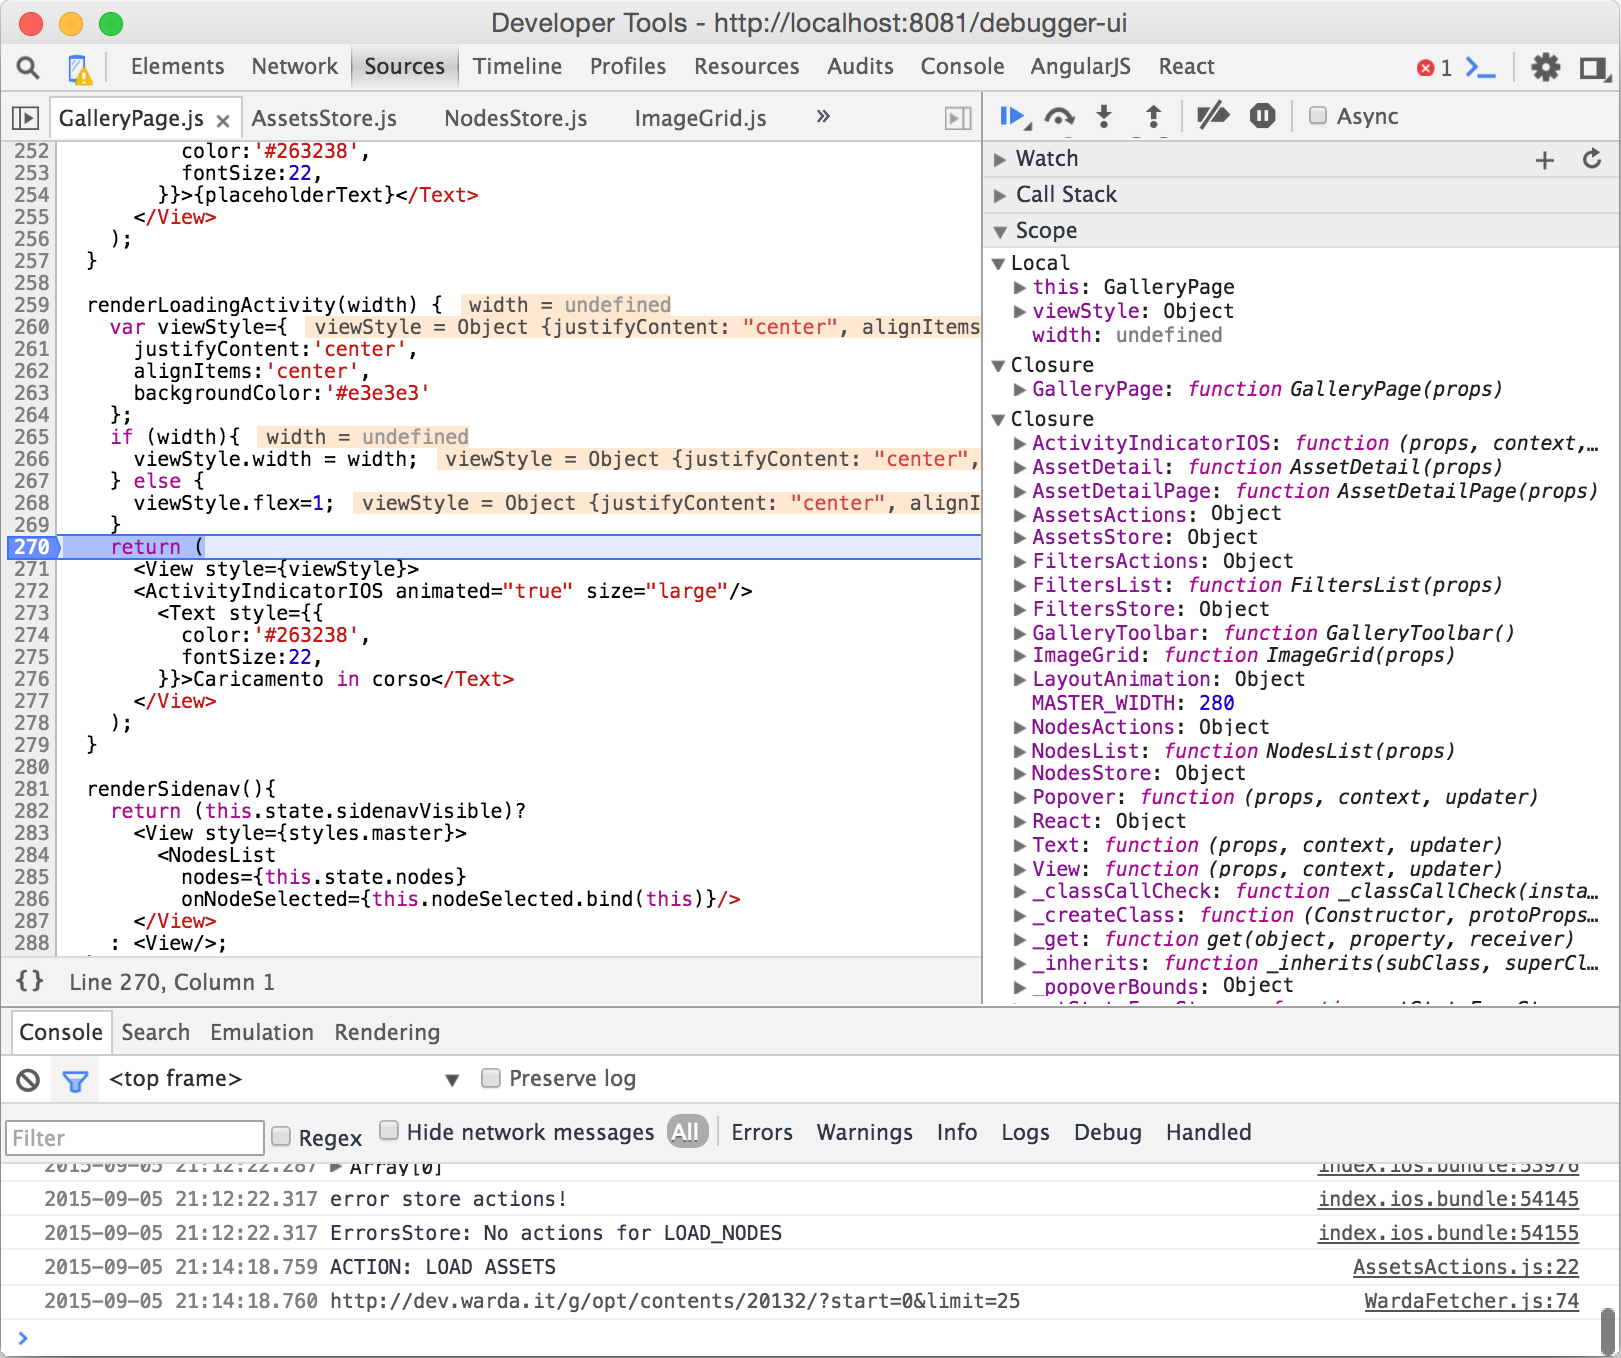
\includegraphics[width=\textwidth]{../immagini/chrome-tools}
\caption{Debug di un'applicazione con Google Chrome}  
\end{figure}

Per avviare il debug è sufficiente preme \texttt{Cmd}+\texttt{D} e selezionare l'opzione \textit{Debug in Chrome}









